% One results figure, two panels. All counts are generated from retained evidence.
% Ordinary manuscript content: no BAJ or MES annotation/highlight commands.
\begingroup
% Generated from preserved evidence by tools/verify_results_figure.py --write-data.
\def\FigSourceDetected{2}
\def\FigSourceMissed{14}
\def\FigSourceProblemTotal{16}
\def\FigSourceExtraFlags{2}
\def\FigSourceFlagTotal{4}
\def\FigSourceRecallPct{12.5}
\def\FigSourcePrecisionPct{50}
\def\FigConditionEligible{10}
\def\FigConditionFlags{5}
\def\FigVisibilitySupported{2}
\def\FigVisibilityDisputed{3}
\def\FigVisibilityPrecisionPct{40}
\def\FigReaderSupported{5}
\def\FigReaderPrecisionPct{100}
\def\FigConditionOther{5}
\def\FigConditionRecallPct{100}
\def\FigCaseOne{C02}
\def\FigCaseTwo{C10}
\def\FigCaseThree{C01}
\def\FigCaseFour{C12}
\def\FigCaseFive{C26}

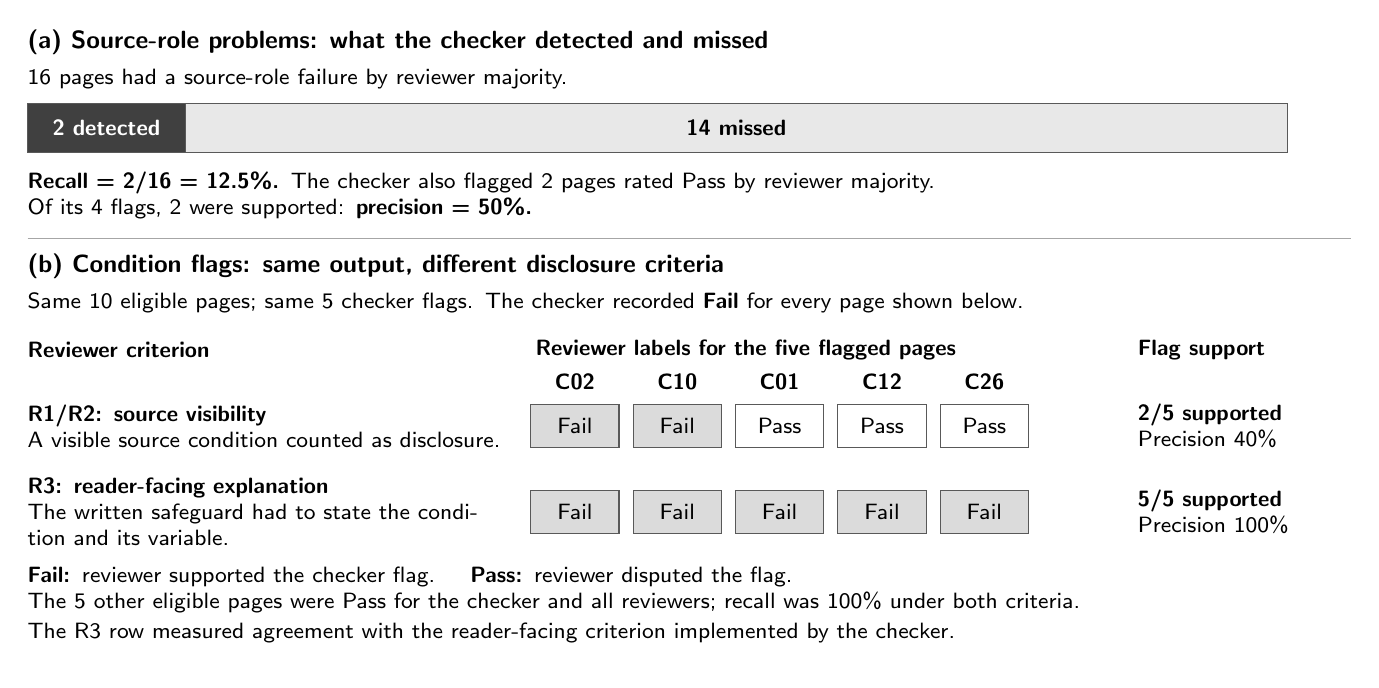
\begin{tikzpicture}[x=1cm,y=1cm,
  font=\sffamily\footnotesize,
  every node/.style={inner sep=0pt,outer sep=0pt},
  heading/.style={anchor=west,font=\sffamily\small\bfseries},
  note/.style={anchor=north west,align=left,text width=16.6cm},
  cell/.style={draw=black!65,minimum width=1.12cm,minimum height=.55cm,font=\sffamily\footnotesize},
  support/.style={cell,fill=black!14},
  disputed/.style={cell,fill=white}
]
\path[use as bounding box] (0,-7.85) rectangle (16.8,.18);

\node[heading] at (0,0) {(a) Source-role problems: what the checker detected and missed};
\node[note] at (0,-.35) {\FigSourceProblemTotal{} pages had a source-role failure by reviewer majority.};
\pgfmathsetmacro{\detectedwidth}{16*\FigSourceDetected/\FigSourceProblemTotal}
\draw[fill=black!75,draw=black!65] (0,-1.4) rectangle (\detectedwidth,-.78);
\draw[fill=black!9,draw=black!65] (\detectedwidth,-1.4) rectangle (16,-.78);
\node[white,align=center,font=\sffamily\footnotesize\bfseries] at ({\detectedwidth/2},-1.09) {\FigSourceDetected{} detected};
\node[align=center,font=\sffamily\footnotesize\bfseries] at ({(\detectedwidth+16)/2},-1.09) {\FigSourceMissed{} missed};
\node[note] at (0,-1.65) {\textbf{Recall = \FigSourceDetected/\FigSourceProblemTotal{} = \FigSourceRecallPct\%.}
  The checker also flagged \FigSourceExtraFlags{} pages rated Pass by reviewer majority.\par
  Of its \FigSourceFlagTotal{} flags, \FigSourceDetected{} were supported: \textbf{precision = \FigSourcePrecisionPct\%.}};

\draw[black!35] (0,-2.5)--(16.8,-2.5);
\node[heading] at (0,-2.85) {(b) Condition flags: same output, different disclosure criteria};
\node[note] at (0,-3.19) {Same \FigConditionEligible{} eligible pages; same \FigConditionFlags{} checker flags.
  The checker recorded \textbf{Fail} for every page shown below.};

\node[anchor=west,font=\sffamily\footnotesize\bfseries] at (0,-3.91) {Reviewer criterion};
\node[anchor=west,font=\sffamily\footnotesize\bfseries] at (6.45,-3.91) {Reviewer labels for the five flagged pages};
\node[anchor=west,font=\sffamily\footnotesize\bfseries] at (14.1,-3.91) {Flag support};
\foreach \x/\cid in {6.95/\FigCaseOne,8.25/\FigCaseTwo,9.55/\FigCaseThree,10.85/\FigCaseFour,12.15/\FigCaseFive}{
  \node[font=\sffamily\footnotesize\bfseries] at (\x,-4.32) {\cid};
}
\node[anchor=west,align=left,text width=6.1cm] at (0,-4.88)
  {\textbf{R1/R2: source visibility}\par A visible source condition counted as disclosure.};
\node[support] at (6.95,-4.88) {Fail};
\node[support] at (8.25,-4.88) {Fail};
\node[disputed] at (9.55,-4.88) {Pass};
\node[disputed] at (10.85,-4.88) {Pass};
\node[disputed] at (12.15,-4.88) {Pass};
\node[anchor=west,align=left,text width=2.6cm] at (14.1,-4.88)
  {\textbf{\FigVisibilitySupported/\FigConditionFlags{} supported}\par Precision \FigVisibilityPrecisionPct\%};

\node[anchor=west,align=left,text width=6.1cm] at (0,-5.97)
  {\textbf{R3: reader-facing explanation}\par The written safeguard had to state the condition and its variable.};
\foreach \x in {6.95,8.25,9.55,10.85,12.15}{\node[support] at (\x,-5.97) {Fail};}
\node[anchor=west,align=left,text width=2.6cm] at (14.1,-5.97)
  {\textbf{\FigReaderSupported/\FigConditionFlags{} supported}\par Precision \FigReaderPrecisionPct\%};

\node[note] at (0,-6.67) {\textbf{Fail:} reviewer supported the checker flag.
  \quad\textbf{Pass:} reviewer disputed the flag.\par
  The \FigConditionOther{} other eligible pages were Pass for the checker and all reviewers; recall was \FigConditionRecallPct\% under both criteria.};
\node[note] at (0,-7.38) {The R3 row measured agreement with the reader-facing criterion implemented by the checker.};
\end{tikzpicture}
\endgroup
